% Required packages for CSV import
% Add these to your document preamble:
% \usepackage{csvsimple}
% \usepackage{longtable}
% \usepackage{array}
% \usepackage{booktabs}

\chapter{Project Initiation}
\minitoc

\section{Introduction}

This project aims to develop a comprehensive PlantUML-based diagramming platform that combines individual productivity tools with community collaboration features. The platform serves as a web-based solution for creating, editing, and sharing PlantUML diagrams while fostering a collaborative environment where users can explore, learn from, and build upon each other's work.

The primary motivation behind this project stems from the need for an integrated platform that not only provides powerful diagramming capabilities but also incorporates modern features such as AI-assisted code editing and community-driven learning. The platform targets developers, software architects, system designers, and educational institutions who require efficient tools for creating technical diagrams and visual documentation.

Key objectives of this project include:
\begin{itemize}
    \item Developing a user-friendly web interface for PlantUML diagram creation and editing
    \item Implementing robust project and diagram management capabilities
    \item Creating a collaborative workspace with AI-powered assistance
    \item Building a community platform for sharing and discovering diagrams
    \item Ensuring scalable architecture with proper authentication and administration features
\end{itemize}

The project follows agile development methodologies using Scrum framework, ensuring iterative development and continuous stakeholder feedback integration.

\section{Analysis and Specification of Requirements}

\subsection{Identification of Actors}

Through comprehensive analysis of the system requirements and user stories, we have identified the following actors who will interact with the PlantUML platform:

\paragraph{Primary Actors (Human Users):}
\begin{itemize}
    \item \textbf{User}: Authenticated individuals who can create, manage, and share diagrams and projects. They have full access to the platform's features including workspace management, community interaction, and profile customization.
    
    \item \textbf{Visitor}: Unauthenticated users who have limited access to the platform. They can explore the landing page and browse community content but cannot create or modify diagrams.
    
\end{itemize}

\paragraph{Secondary Actors (System Components):}
\begin{itemize}
    \item \textbf{AI System}: An intelligent assistant that responds to user requests and provides code editing assistance for diagram creation and modification.
    
    \item \textbf{PlantUML Server}: External service responsible for rendering PlantUML code into visual diagram representations.
\end{itemize}

\subsection{Identification of Requirements}

\subsubsection{Functional Requirements}

The functional requirements have been categorized based on the main feature areas of the platform:

\paragraph{Authentication and Security:}
\begin{itemize}
    \item Support for OAuth authentication via Google and GitHub accounts
    \item Cross-device authentication persistence
    \item Secure logout functionality
    \item Administrative authentication with elevated privileges
\end{itemize}

\paragraph{Project and Diagram Management:}
\begin{itemize}
    \item Complete CRUD operations for projects and diagrams
    \item Project organization and categorization capabilities
    \item Bulk download functionality for project diagrams
    \item Individual diagram export in multiple formats
    \item Project sharing and collaboration features
\end{itemize}

\paragraph{Workspace and Editing:}
\begin{itemize}
    \item Interactive code editor for PlantUML syntax
    \item Split-view workspace with customizable layouts
    \item Real-time diagram rendering and preview
    \item AI-powered code assistance and suggestions
    \item Syntax highlighting and error detection
\end{itemize}

\paragraph{Community Features:}
\begin{itemize}
    \item Public project exploration and discovery
    \item Comment system with full CRUD operations
    \item Like/unlike functionality for projects and comments
    \item Project forking and copying capabilities
    \item Social sharing features
\end{itemize}

\paragraph{Profile:}
\begin{itemize}
    \item User profile management and customization
    \item Public project portfolio display
 \end{itemize}

\subsubsection{Non-Functional Requirements}

\paragraph{Performance Requirements:}
\begin{itemize}
    \item Page load times should not exceed 3 seconds under normal conditions
    \item Diagram rendering should complete within 5 seconds for standard-sized diagrams
    \item The system should support concurrent access by up to 1000 users
    \item Real-time editor updates should have latency below 100ms
\end{itemize}

\paragraph{Security Requirements:}
\begin{itemize}
    \item All data transmission must be encrypted using HTTPS/TLS
    \item User authentication must follow OAuth 2.0 security standards
    \item Input validation and sanitization for all user-generated content
    \item Protection against common web vulnerabilities (XSS, CSRF, SQL injection)
\end{itemize}

\paragraph{Usability Requirements:}
\begin{itemize}
    \item Intuitive user interface following modern web design principles
    \item Responsive design supporting desktop, tablet, and mobile devices
    \item Accessibility compliance with WCAG 2.1 Level AA standards
    \item Multilingual support with initial focus on English
\end{itemize}

\paragraph{Reliability and Availability:}
\begin{itemize}
    \item System uptime of 99.5\% excluding scheduled maintenance
    \item Automated backup systems with 24-hour recovery point objective
    \item Graceful error handling with meaningful user feedback
    \item Fault tolerance for external service dependencies
\end{itemize}

\paragraph{Scalability Requirements:}
\begin{itemize}
    \item Horizontal scaling capability for increased user load
    \item Database optimization for efficient query performance
    \item CDN integration for static asset delivery
    \item Microservices architecture for independent component scaling
\end{itemize}

\section{Project Management with Scrum}

\subsection{Scrum Roles}

The project adopts the Scrum framework with clearly defined roles and responsibilities:

\paragraph{Roles in the Scrum Team:}

\begin{table}[h!]
    \centering
    \begin{tabular}{|l|l|}
        \hline
        \textbf{Role}          & \textbf{Member(s)}             \\ \hline
        Product Owner          & Issam Mekni                   \\ \hline
        Scrum Master           & Issam Mekni                   \\ \hline
        Development Team       & Issam Mekni, Souhaieb Askri   \\ \hline
    \end{tabular}
    \caption{Scrum roles and their respective members}
\end{table}


\subsection{Product Backlog}

The product backlog represents a prioritized list of features and requirements derived from stakeholder needs and market analysis. Each backlog item follows the user story format and includes priority classification using MoSCoW method (Must have, Should have, Could have, Won't have this time).

% Automatic CSV import for Product Backlog using longtable
\begin{longtable}{|p{0.7cm}|p{3.6cm}|p{0.7cm}|p{9cm}|p{1.5cm}|}
\caption{Product Backlog with User Stories and Priorities (Imported from backlog.csv)} \label{tab:product_backlog} \\
\hline
\textbf{ID} & \textbf{Feature} & \textbf{Sub-ID} & \textbf{User Story} & \textbf{Priority} \\
\hline
\endfirsthead

\multicolumn{5}{c}%
{{\bfseries \tablename\ \thetable{} -- continued from previous page}} \\
\hline
\textbf{ID} & \textbf{Feature} & \textbf{Sub-ID} & \textbf{User Story} & \textbf{Priority} \\
\hline
\endhead

\hline \multicolumn{5}{|r|}{{Continued on next page}} \\ \hline
\endfoot

\hline
\endlastfoot

\csvreader[no head, late after line=\\]{./backlog1.csv}{}%
{\csvcoli & \csvcolii & \csvcoliii & \csvcoliv & \csvcolv}
\end{longtable}

\subsection{Global Use Case Diagram}

The global use case diagram provides a comprehensive overview of the system's functionality and actor interactions. It illustrates the relationships between different use cases and demonstrates how various actors engage with the platform's features.

\begin{figure}[H]
    \centering
    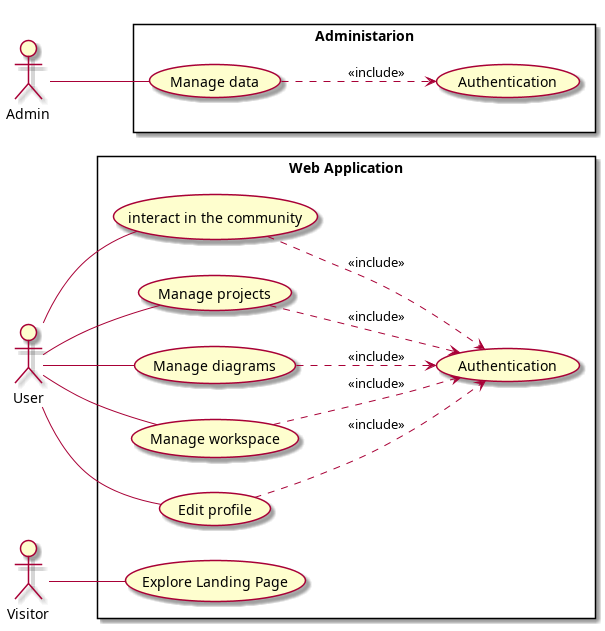
\includegraphics[width=\textwidth]{./conception/global_use_case_diagram.png}
    \caption{Global Use Case Diagram}
    \label{fig:global_use_case}
\end{figure}

% The diagram showcases the following key aspects:
% \begin{itemize}
%     \item \textbf{Actor Separation}: Clear distinction between primary actors (User, Visitor, Admin) and secondary actors (AI System, PlantUML Server)
%     \item \textbf{Package Organization}: Logical grouping of related use cases into coherent packages
%     \item \textbf{Relationship Modeling}: Proper use of include, extend, and generalization relationships
%     \item \textbf{System Boundary}: Clear delineation of system scope and external dependencies
% \end{itemize}

\subsection{Sprint Planning}

The project is organized into six strategic sprints, each focusing on specific functional areas and building upon previous deliverables. The total project duration is designed to fit within 3.5 months (14 weeks) with efficient resource allocation and parallel development activities.

\begin{table}[h!]
    \centering
    \begin{tabular}{|c|l|l|c|}
        \hline
        \textbf{Sprint} & \textbf{Focus Area}                                & \textbf{Backlog Features}                                   & \textbf{Weeks} \\ \hline
        I              & Infrastructure Setup                               & N/A                                                     & 2                                   \\ \hline
        II             & Authentication and Landing Page                    & 1,2                              & 2                                   \\ \hline
        III            & Project Management                                 & 3                            & 3                                   \\ \hline
        IV             & Diagram and Project Management                     & 4,5                            & 3                                   \\ \hline
        V              & Community Interaction and Profiles                 & 6 ,7                          & 3                                   \\ \hline
    \end{tabular}
    \caption{Scrum Sprint Planning with Estimated Durations}
\end{table}

\section{Deployment diagram}

The deployment diagram illustrates the system's architecture at the deployment level, showing how components are deployed and how they interact with external systems and services.

\begin{figure}[H]
    \centering
    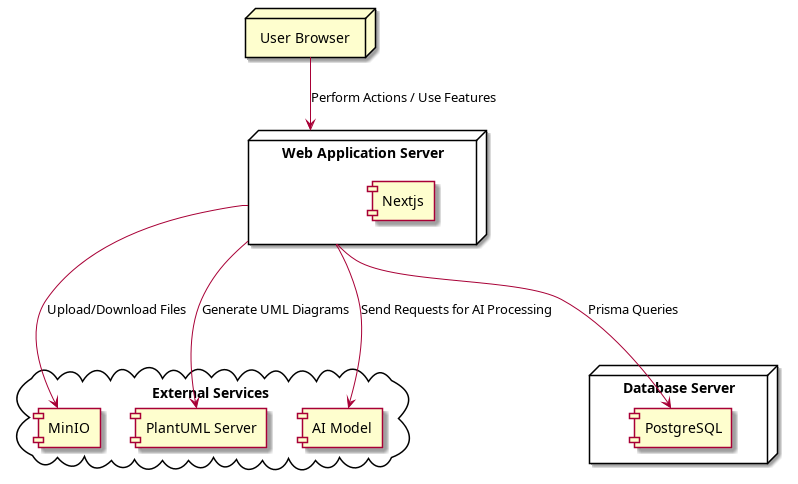
\includegraphics[width=\textwidth]{./conception/deployement_diagram.png}
    \caption{Deployment diagram}
    \label{fig:deployment}
\end{figure}

\section{Technological Architecture of the Project}
% This section will be detailed in subsequent documentation phases.

\section{Tools and Environment}
The development of the platform leverages a modern web technology stack, development tools, and runtime environments that support scalable, maintainable, and collaborative software engineering practices.

\begin{longtable}{|m{3.5cm}|m{4cm}|m{6.5cm}|}
    \caption{Tools and Environment Used in the Project (Ordered by Usage)} \label{tab:tools_env_ordered} \\
    \hline
    \textbf{Tool/Technology} & \textbf{Logo} & \textbf{Purpose} \\
    \hline
    \endfirsthead
    
    \hline
    \textbf{Tool/Technology} & \textbf{Logo} & \textbf{Purpose} \\
    \hline
    \endhead
    
    \endfoot
    
    \hline
    \endlastfoot
    Linux & 
\includegraphics[width=1.5cm]{pictures/web/logo/linux.png} & Operating system environment for development and deployment \\
    \hline
    Git & 
\includegraphics[width=1.5cm]{pictures/web/logo/git.png} & Distributed version control system \\
    \hline
    GitHub & 
\includegraphics[width=1.5cm]{pictures/web/logo/github-mark.png} & Version control and collaborative code hosting \\
    \hline
    VSCodium & 
\includegraphics[width=1.5cm]{pictures/web/logo/vscodium-icon.png} & Open-source code editor used for development \\
    \hline
    LaTeX & 
\includegraphics[width=1.5cm]{pictures/web/logo/latex.png} & Document preparation system for high-quality typesetting \\
    \hline
    Node.js & 
\includegraphics[width=1.5cm]{pictures/web/logo/node-svgrepo-com.png} & JavaScript runtime for backend services \\
    \hline
    Next.js & 
\includegraphics[width=1.5cm]{pictures/web/logo/next-js.png} & React framework for server-side rendering and routing \\
    \hline
    React & 
\includegraphics[width=1.5cm]{pictures/web/logo/reactts-svgrepo-com.png} & JavaScript library for building user interfaces \\
    \hline
    TypeScript & 
\includegraphics[width=1.5cm]{pictures/web/logo/typescript-official-svgrepo-com.png} & Static typing for JavaScript to enhance code quality \\
    \hline
    NextAuth.js & 
\includegraphics[width=1.5cm]{pictures/web/logo/next-authe.png} & Authentication library for Next.js applications \\
    \hline
    Tailwind CSS & 
\includegraphics[width=1.5cm]{pictures/web/logo/tailwind-svgrepo-com.png} & Utility-first CSS framework for fast UI development \\
    \hline
    ShadCN/UI & 
\includegraphics[width=1.5cm]{pictures/web/logo/shad-cn-ui.png} & Component library built on top of Tailwind for accessible UI components \\
    \hline
    Prisma & 
\includegraphics[width=1.5cm]{pictures/web/logo/prisma.png} & ORM for database access and modeling \\
    \hline
    PostgreSQL & 
\includegraphics[width=1.5cm]{pictures/web/logo/pgsql-svgrepo-com.png} & Relational database used for storing platform data \\
    \hline
    Express.js & 
\includegraphics[width=1.5cm]{pictures/web/logo/express-js.png} & Web server for handling API routes and middleware \\
    \hline
    LangChain & 
\includegraphics[width=1.5cm]{pictures/web/logo/langchain-icon-seeklogo.png} & Framework for developing AI-driven assistant features \\
    \hline
    PlantUML & 
\includegraphics[width=1.5cm]{pictures/web/logo/plantuml-svgrepo-com.png} & Tool for creating UML diagrams from plain text \\
    \hline
    AdminJS & 
\includegraphics[width=1.5cm]{pictures/web/logo/admin-js.png} & Admin panel framework for managing application data \\
    \hline
    Docker & 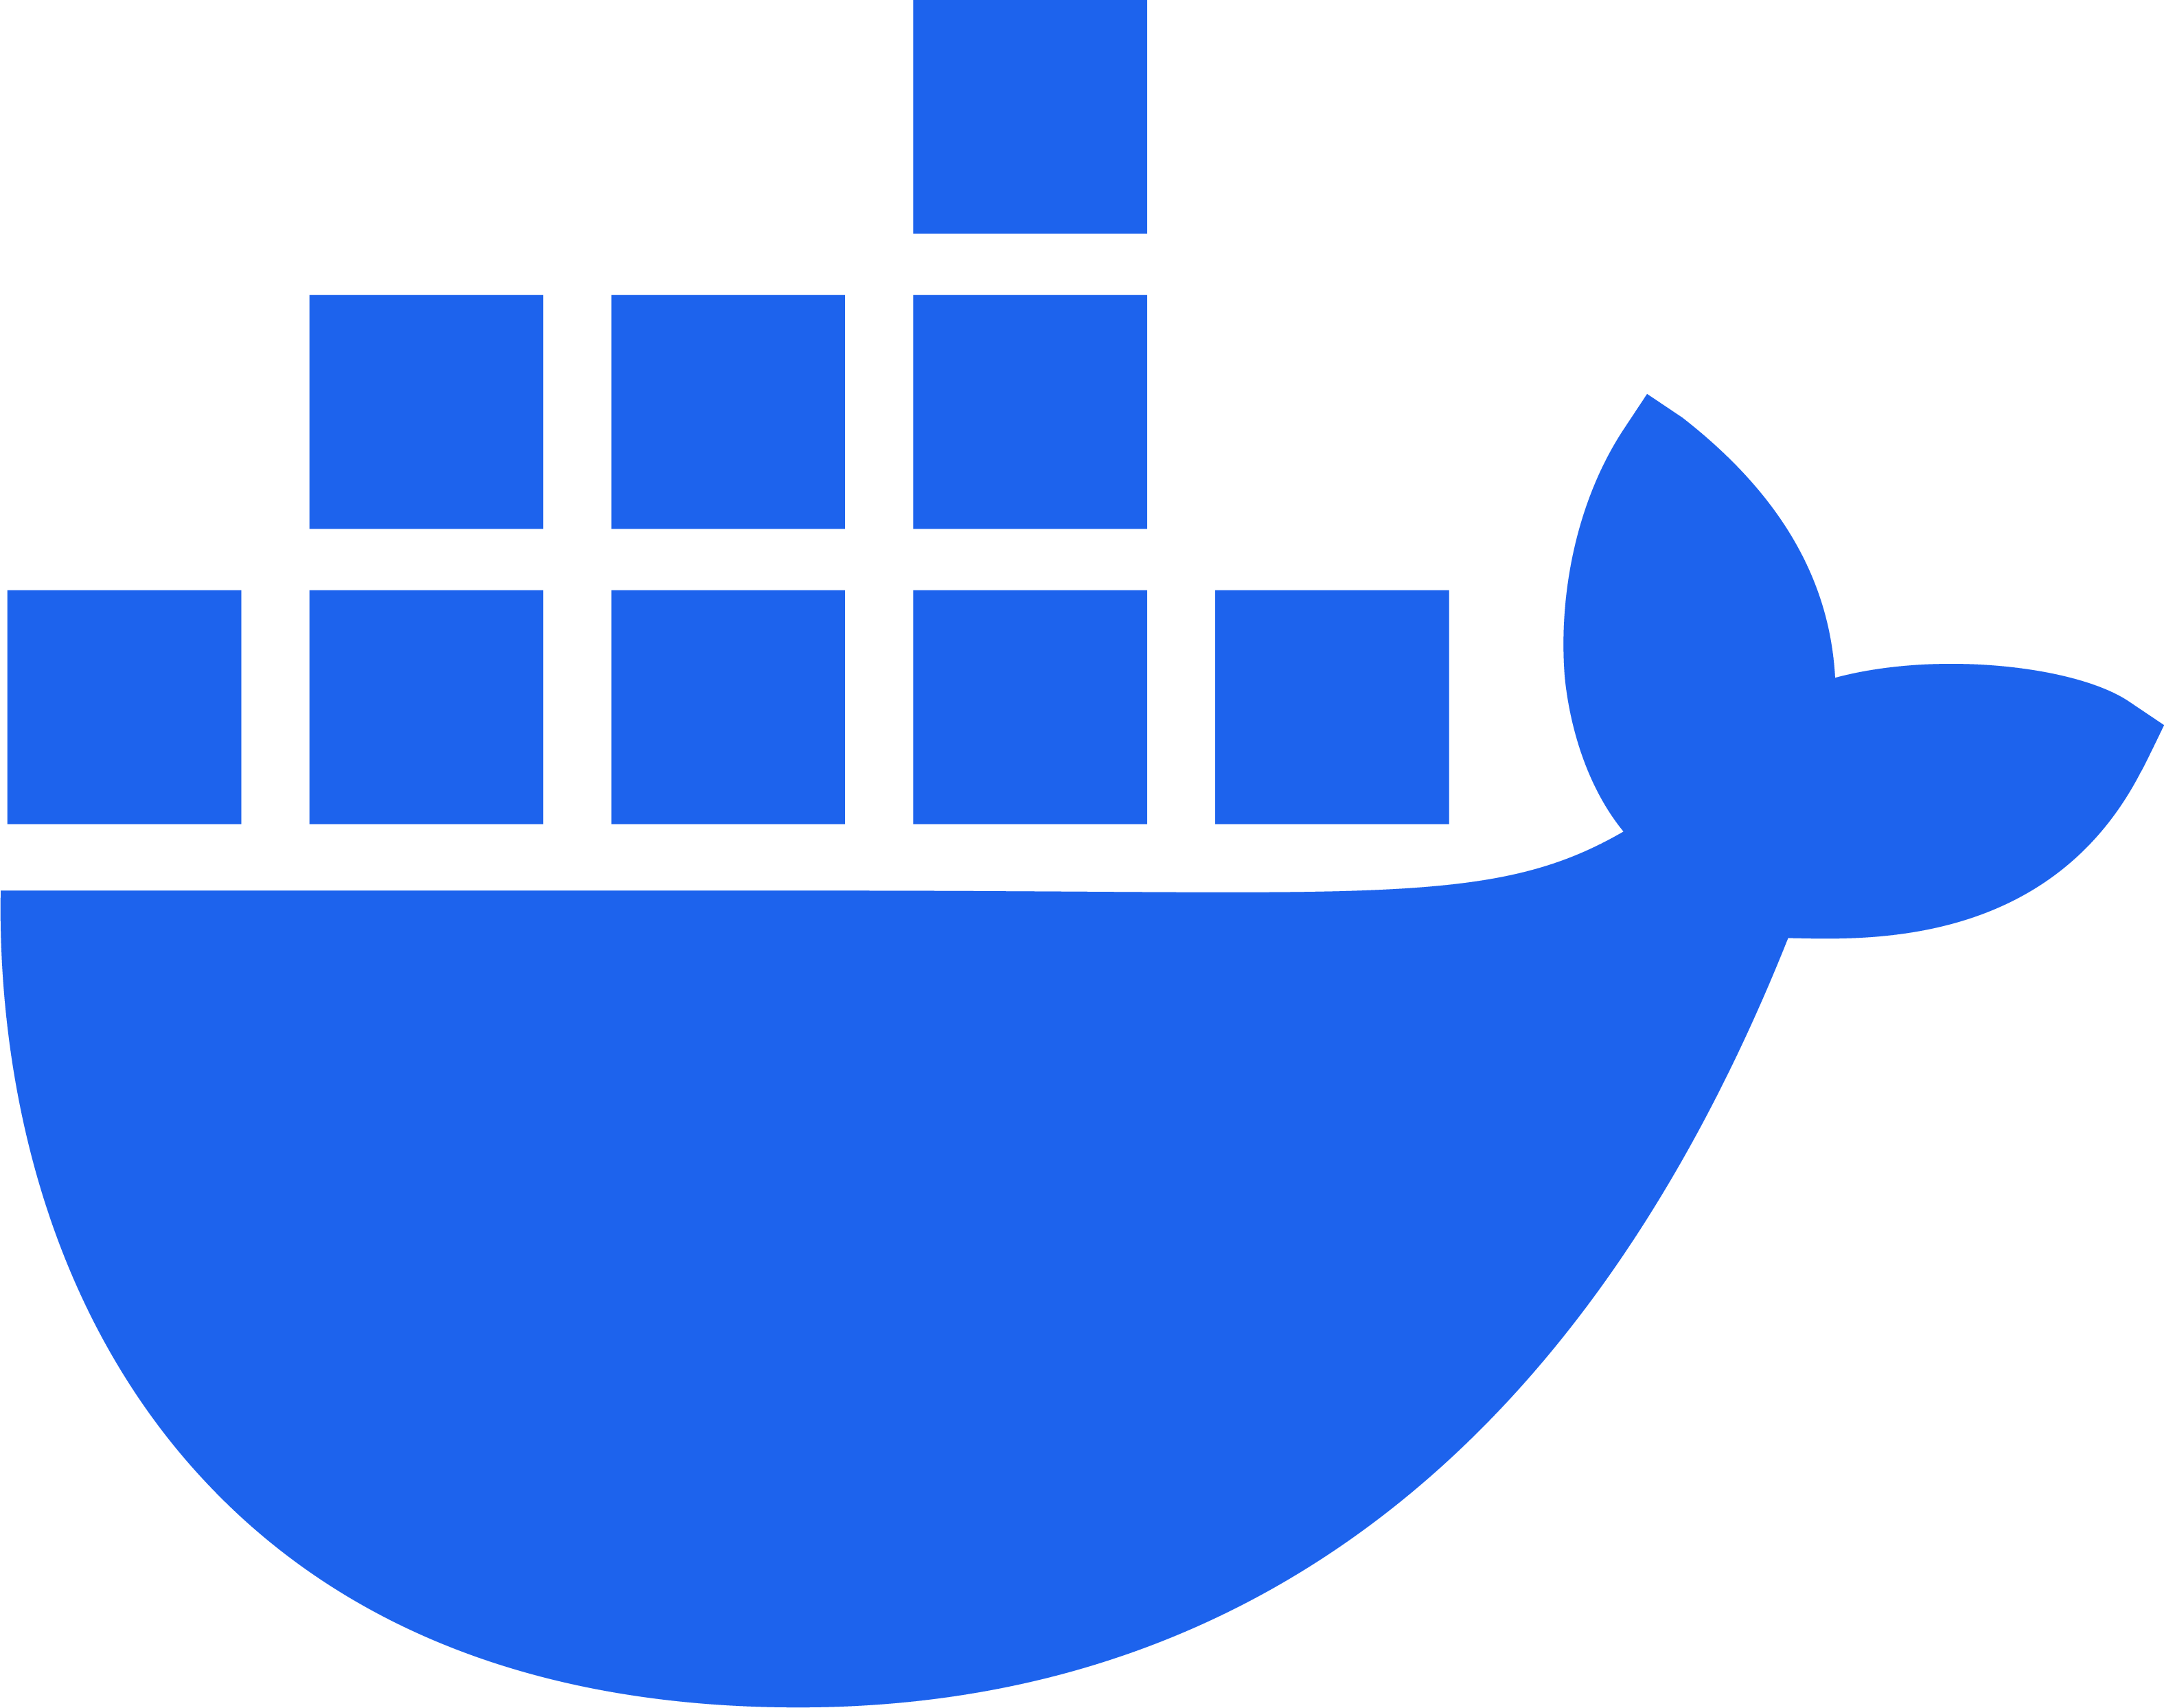
\includegraphics[width=1.5cm]{pictures/web/logo/docker.png} & Containerization platform for application deployment \\
    \hline
    MinIO & 
\includegraphics[width=1.5cm]{pictures/web/logo/minio.png} & Object storage server compatible with Amazon S3 API \\
    \hline
    Firefox & 
\includegraphics[width=1.5cm]{pictures/web/logo/firefox.png} & Browser used for development and testing \\
    \hline
    \end{longtable}
       
    
% This section will be detailed in subsequent documentation phases.

\section{Conclusion}

The project initiation phase has established a solid foundation for the development of the platform through comprehensive requirement analysis, stakeholder identification, and strategic planning. The adoption of Scrum methodology ensures iterative development with regular feedback incorporation and continuous improvement.

Key achievements of this initiation phase include:
\begin{itemize}
    \item Clear identification of system actors and their interactions
    \item Comprehensive functional and non-functional requirements specification
    \item Well-structured product backlog with prioritized user stories
    \item Detailed sprint planning with realistic timelines and deliverables
    \item Established project management framework using Scrum principles
\end{itemize}

The systematic approach to requirement gathering and analysis has revealed the complexity and scope of the platform while ensuring that all stakeholder needs are addressed. The priority-based classification of requirements enables focused development on core functionality while maintaining flexibility for future enhancements.

The sprint-based development approach provides clear milestones and deliverables, facilitating progress tracking and stakeholder communication. The incremental nature of the development process allows for early feedback integration and risk mitigation.

Moving forward, the project is well-positioned to proceed with the technical architecture design and implementation phases, building upon the solid foundation established during this initiation phase. The comprehensive documentation created during this phase will serve as a reference throughout the development lifecycle, ensuring consistency and alignment with project objectives.